\chapter{NEUCOGAR, организация моторного вывода}
\label{chap:literature_review}

\section{NEUCOGAR}
Базисом когнитивных архитектур является предположение, что функциональные аспекты мышления человека можно описать на уровне вычислений и воспроизвести в машине на принципах, не требующих детального моделирования нейронов и структур мозга. 
В первую очередь: 
\begin{itemize}
	\item принципы восприятия информации
	\item осмысление информации
	\item принятие и исполнение решений
\end{itemize}

Ключевыми при таком подходе являются принципы социального и эмоционального интеллекта.
Создание и осознание в машине аналога человеческого субъекта на этих принципах может привести к технологическому прорыву и созданию , который окажет огромное влияние на жизнь человека.

Целю NEUCOGAR является моделирование влияния серотонина, дофамина и норадреналина на симуляции мозга, основанные на архитектуре фон Неймана. 
И реализовать данные явления в виде на модели, исполнимой в машине Тьюринга. В качестве основы моделирования используется расширенный Куб эмоций Лёвхейма. Валидация проводится путем моделирования на вычислительной системе нейромодуляции дофамина и ее влияния на кору.


\section{Организация моторного вывода}
\label{section:motor_things}
\subsection{Моторная кора}
Моторная кора является областью коры головного мозга, которая участвует в планировании, контроле и выполнении добровольных движений. 
Она представляет собой область лобной доли, расположенную в задней прецентральной извилине, непосредственно перед центральной борозды.~\cite{wiki:motor}
Компоненты моторной коры:

\begin{itemize}
	\item первичная моторная зона --- основной источник нейронных импульсов, которые проходят вниз по спинному мозгу и контролируют выполнение движения
	\item премоторная зона отвечает за некоторые аспекты управления движением, включая подготовку к ней, оркестровку и пространственное наведение на достижение цели
	\item дополнительная моторная область --- внутреннее планирование движения, последовательности и координацию исполнения движений
\end{itemize}
Задняя теменная кора иногда также считается частью группы кортикальных областей.
Она несет ответственность за интеграцию сенсорной информации в моторные команды и за некоторые аспекты моторного планирования.~\cite{motorcortex}

Двигательная кора в целом --- это мозаика двигательных групп нейронов, относящихся к определенным группам мышц. Данные группы организованы соматотопически и в совокупности составляют схематичное отображение тела человека на коре мозга, называемый гомункулус~\ref{fig:homunculus}.
\begin{figure}
	\centering
	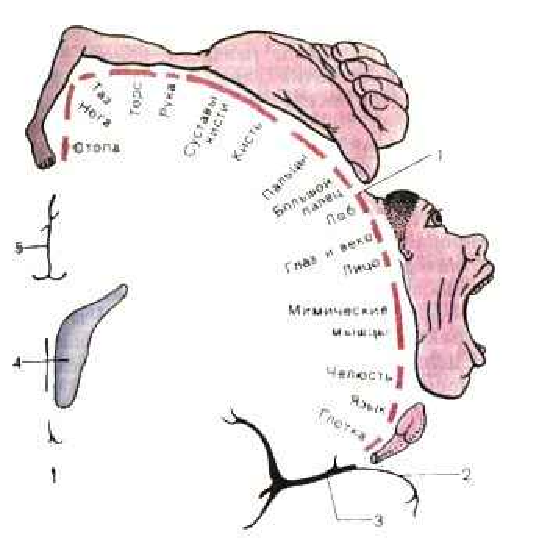
\includegraphics[width=\linewidth/2]{homunculus}
	\caption{Двигательный гомункулус. }
	\label{fig:homunculus}
\end{figure}

\subsection{Ствол головного мозга}
Ствол мозга при помощи серого вещества обеспечивает многие основные функции для выживания организма, кроме того, исполняет рефлексы. Он состоит из нескольких структурных элементов: 
\begin{itemize}
	\item средний мозг
	\item Варолиев мост
	\item продолговатый мозг
\end{itemize}
Белое вещества мозгового ствола образует связи между мозгом и телом через спинной мозг, в том числе:
\begin{itemize}
	\item кортикоспинальный тракт для передачи сигналов мышцам для исполнения движений
	\item cпиноталамический тракт для сигнализации боли, зуда и других стимулов
\end{itemize}

Ретикулярная формация, которая распространяется по всему стволу мозга, выполняет несколько важных функций, включая стимуляцию коры головного мозга и поддержку мышечного тонуса. 
Стимуляция коры головного мозга ретикулярной формацией вызывает эффект бодрствования и сознания, тогда как инактивация ретикулярной формации приводит к сну.

Через продолговатый мозг проходят все нейроны, соединяющие мозг со спинным мозгом, и на уровне продолговатого мозга около 90\% этих нейронов перемещаются с левой стороны тела вправо и наоборот.~\cite{corticospinal}
Хотя причина этого явления неизвестна, оно объясняет, почему мозг чувствует и контролирует контралатеральную сторону тела. 
Эти нейроны, проходящие через продолговатый мозг, также множество раз передают свой сигнал другому нейрону, который несет сигнал дальше к мозгу или телу. 
Ядра серого вещества в продолговатом мозге включают сердечно-сосудистый центр, который контролирует сердечный ритм и кровяное давление, а также область, которая контролирует скорость дыхания. 
Многие жизненные рефлексы интегрированы в продолговатый мозг, в том числе рефлексы глотания, рвоты и кашля.

Подобно продолговатому мозгу, Варолиев мост(в дальнейшем мост) играет важную роль в коммуникациях, так как содержит нейроны, которые соединяют более высокие области мозга с продолговатым мозгом и спинным мозгом.

\subsection{Основные проводящие пути}
Добровольные движения верхней конечности происходят в основном из контрлатеральной моторной коры, которая получает входные сигналы от лобной и теменной областей, которые играют важную роль в сенсомоторной обработке. 
Моторные области коры мозга плотно взаимосвязаны в пределах одного полушария через связные пути и соединяются с гомологичными областями противоположного полушария.

Кортикоспинальный тракт является основным двигательным путем. 
Он образован большими пирамидальными нейронами из первичной моторной зоны. 
Тракт проходит через весь головной мозг и в нижней части продолговатого мозга примерно 90\% его волокон переходит на противоположную сторону, формируя боковой пирамидный тракт.
Остальные волокна спускаются в спинной мозг, не пересекаясь.
Считается, что эти непересеченные передние выступы главным образом иннервируют проксимальные мышцы, а не дистальные мышцы предплечья и руки.~\cite{cnsphysiology}

Афферентный кортикальный вход, необходимый для точного выполнения движений, доставляет сенсорную информацию через таламокортикальное пути в двигательные области и первичную и вторичную сенсорные области. 
Обзор соответствующих трактов и структур, связанных с сенсомоторной функцией конечностей, представлен на рис.~\ref{fig:connections}.
\begin{figure}
	\centering
	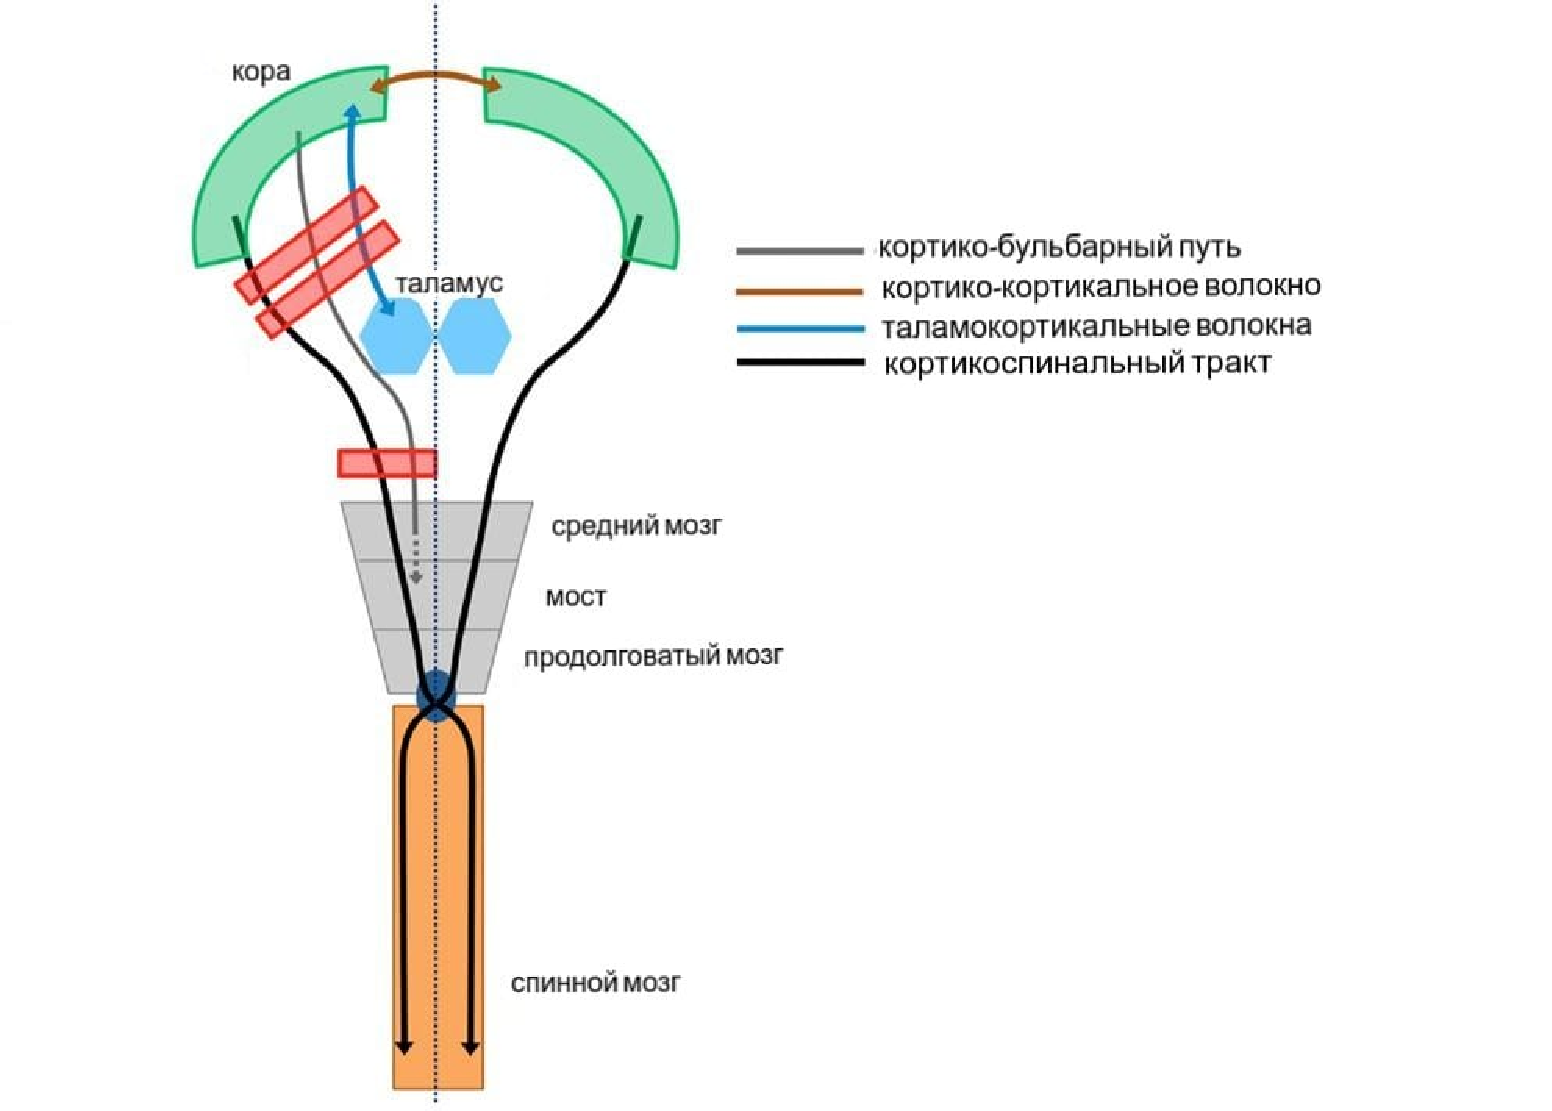
\includegraphics[width=\linewidth]{overview}
	\caption{Структурная связность моторной системы. }
	\label{fig:connections}
\end{figure}